\documentclass[10pt]{article}
%\documentclass[review]{siamart0516}
%\usepackage[utf8]{inputenc}
\usepackage[T1]{fontenc}
\usepackage{lmodern}
\usepackage{subfig}
%\usepackage[latin1]{inputenc}
\usepackage[english]{babel}
\usepackage{fullpage}
\usepackage{multirow}
%\usepackage{amsmath,amssymb,psfrag, amsthm}
\usepackage{amsmath,amssymb,psfrag}
\usepackage{graphicx}
\usepackage{listings}
\usepackage{paralist}
\usepackage{appendix}
%\usepackage{natbib}
\usepackage{amsfonts}
\usepackage{subfig,color}
\usepackage{comment} 
\usepackage{enumerate}
\usepackage{cancel}
%\usepackage{helvet}
%\usepackage{algorithm}
%\usepackage{algorithmicx}
%\usepackage{algpseudocode}
\usepackage{epstopdf}
\usepackage{tikz,tikz-cd}
\usepackage{listings}
\usepackage{pgfplots,pgfplotstable}
\usetikzlibrary{pgfplots.groupplots}
\usetikzlibrary{positioning}
\usetikzlibrary[shapes,arrows,trees]
\usetikzlibrary{matrix,decorations.pathmorphing}
%\newcommand{\refalg}[1]{Algorithm~\ref{#1}}
%\newcommand{\refsec}[1]{Section~\ref{#1}}
%\newcommand{\reffig}[1]{Figure~\ref{#1}}
%\newcommand{\refsubfig}[1]{Figure~\subref{#1}}
%\newcommand{\reftab}[1]{Table~\ref{#1}}
%\newcommand{\refeqn}[1]{(\ref{#1})}
%\newcommand{\reflst}[1]{Listing~(\ref{#1})}
\newcommand{\refalg}[1]{\cref{#1}}
\newcommand{\refsec}[1]{\cref{#1}}
\newcommand{\reffig}[1]{\cref{#1}}
\newcommand{\refsubfig}[1]{\cref{#1}}
\newcommand{\reftab}[1]{\cref{#1}}
\newcommand{\refeqn}[1]{\cref{#1}}
\newcommand{\reflst}[1]{\cref{#1}}
\renewcommand{\d}{\mathrm{d}}
\newcommand{\re}[1]{(\ref{#1})}
\newcommand{\D}{\mathrm{D}}
\newcommand{\bb}[1]{\boldsymbol{#1}}
\def\sgn{\mathop{\rm sgn}}
\newcommand{\remark}[1]{{\color{red} #1}}
% THEOREMS ETC
\newcommand{\vect}[1]{\mathbf{#1} }
\newcommand{\order}[1]{\mathcal{O}(h^{#1})}
\newcommand{\code}[1]{{\tt #1}}
\renewcommand{\familydefault}{\sfdefault}
% -----------------------------------------------------------
% -----------------------------------------------------------
\lstset{backgroundcolor=\color[rgb]{0.92,0.95,1}}
\lstset{rulecolor=\color[rgb]{0.92,0.95,1}}
\lstset{numbers=left}
\lstset{basicstyle=\ttfamily\footnotesize}
\lstset{numberstyle=\footnotesize}

\def\dfdd#1#2{\frac{\partial#1}{\partial#2}}
\newcommand{\erf}{\, \mathrm{erf}}
\newcommand{\erfc}{\, \mathrm{erfc}}
%\renewcommand{\labelenumi}{[\arabic{enumi}]}

\newcommand{\dt}{\Delta t}
\newcommand{\dd}{\:\textrm{d}}
\newcommand{\CostFcn}{J}
\newcommand{\CostIntegrand}{g}
\newcommand{\param}{p}
\newcommand{\PDEConstr}{P}
\newcommand{\ModelN}{{\mathcal{F}}}
\newcommand{\ModelTLM}{F}
\newcommand{\Lagrangian}{{\mathcal{L}}}

%\normalsize

\begin{document}
%\def\thefigure{\arabic{figure}}
%\def\thetable{\arabic{table}}

% TITLE AND AUTHOR --------------------------------
\title{PDE constrained optimization, error estimation and control\footnote{we haven't done control} with spectral elements using PETSc and TAO}
\vspace{1cm}
\author{Oana Marin, Emil Constantinescu, Barry Smith}
\date{\today}
\maketitle

Parameter determination by fitting observations, of either numerical or experimental nature, acceleration of simulations throughout their long transients, identification of boundary conditions that satisfy certain observation, and many more such applications fall within the field of PDE constrained optimization and inverse problems. Despite their widespread usability inverse problems have been plagued by bottlenecks such as: ill-posedness, data intensity, sensitivity to errors, high computational costs. The current work aims to address these issues by leveraging the extensive range of methods available in both PETSc and TAO, to provide a framework for tackling large scale inverse problems in a robust fashion.

%The traditional approach to PDE constrained optimization is mathematically similar to the inverse problems approach however differs in terms of computational 

A PDE constrained optimization problem can be stated in two different ways according to the problem at hand: either by fully discretizing the entire KKT system, as is customary in the optimization community \cite{Haber_2007}, or by decoupling the direct problem and its adjoint and solving them via a forward/backward timestepping loop, with appropiate initial and boundary conditions depending on the objective function.

We aim to adddress three of the five main startegies outlined in \cite{Brown_2008}. Specifically the core strategy in \cite{Brown_2008} is to proceed to the solution of inverse problem in a purely non-linear manner (a lot of work has previously relied on linearizations), and here we showcase a nonlinear time dependent convection problem solved in PETSc with TAO. A second outlined challenge is to identify connections between uncertainty in the model and its underlying mathematical structure. This point can be interpreted in several ways and encompases a series of problems, however we shall address this by means of error analysis of the numerical implementation and its impact on optimization. The last aspect we begin to grapple with is the gap between mathematical research and domain specific expertise, with a direct focus on Computational Fluid Dynamics applications. Since the implementation is performed in the PETSc framework, a byproduct of this work is to open the road to a fourth strategy stated in \cite{Brown_2008}, which refers to the development of large-scale linear algebraic techniques that reliably capture the structure of ill-posedness. 

Given that inverse problems based on the full nonlinear underlying PDE as opposed to linearizations has been an issue for a long time, the data and computational intensity aspect has often been overlooked, however we adressed this in previous work \cite{schanen_2016}. The data intensity for nonlinear problems stems mainly from the nature of the backward in time component which depends at every time instance on its forward counterpart. A robust treatment for balancing the compute time versus trajectory storage has been already implemented in PETSc for certain time stepping routines for ordinary differential equations (cite hong) and in the current work we explore/extend it further to PDEs. 

A known aspect in the PDE optimization community is that continous derivations of the adjoint equation differ in nature from their discrete correspondent, and may subsequently provide a shifted gradient which affects the convergence of the optimization step. To surpass this issue we implemented a spectral element method in PETSc which is the spatial discretization with the highest accuracy per grid point of all presently available numerical schemes. Another novelty factor this work intends to bring about is to equip the solvers with a combined space/time error analysis to facilitate studies on the impact of errors on the optimization step. The relevance of this addition cannot be stressed enough, since the errors in the gradient computation tend to slow the convergence rate of the optimization.

The material is organized as follows: the time dependent inverse problem is stated in a spatially unaware fashion, which allows for any operators such as diffussion, convection etc. As a prerequisite the main aspects of a spectral element method are presented together with a discussion on best implementation choices. A set of canonical test problems is explored in depth by describing the continous adjoint versus the discrete adjoint, followed by an error analysis discussion. Results of the PETSc/TAO implementation are presented, together with an outloook on future work.


  
\section{Inverse problem\label{sec:inverse}}
The aim of this work to estimate and control the error in the solution of PDE constrained optimization problems.
We will denote a generic PDE model by
\begin{eqnarray}
 \frac{\partial u}{\partial t} &=& \mathcal P[ u ] , \  x \in \Omega \\ \nonumber
   B[u|_{\partial \Omega}(t)]&=& u_b(t), \\ \nonumber
   u( x,0)&=& u_0( x),\label{eq:generic}
\end{eqnarray} 
where $\mathcal P[ u ]$ is a stand-in operator for derivatives controlling the spatial behaviour of the solution $u$. The boundary condition $u_b$ is also provided by an operator $B[u]$ which can be the indetity for Dirichlet boundary conditions or a derivative for Neumann, while $u_b(t)$ denotes whether the boundaries are homogenously or inhomogenously satisfied. We draw the attention that this notation does not exclude periodic boundary conditions, which can be inforced by a quasi-identity operator $B[\cdot]$ such that $B[u_0]=u_N$ and $B[u_N]=u_0$, while $B[u_i]=u_i$ for $i=1,\ldots,N-1$ for all $t\in [0,\ T]$.

%Let us assume that we seek to find the initial condition $u_0$ such
that we minimize a function
%
%\begin{align}
%  \label{eq:Cost:general}
%\CostFcn(u_0) = \int_0^T \CostIntegrand(u(t)) \dd t\,.
%\end{align}
%

In this work we will consider simple data assimilation problems  for which we seek the initial condition $u_0$ that leads at time $T$ to a solution
$u$ which matches a reference solution $u_d$. Typically $ u_d$  is not known over the entire domain $\Omega$
in practice, but in a subset region $\Omega_s$ where sensors have been
placed. However, for simplicity we construct a continuous function
$\mathbf u_d$ to avoid regularization issues. 
A cost function which minimizes the difference between $| u- u_d|$ while preserving convexity is
$$J[u|_T]=\int_{\Omega}(u(T)- u_d(T))^2 \ \d \Omega \,. $$


We seek $u_0$ initial condition which satisfies Eq.~\ref{eq:generic} such that $J[ u|_T]$ is minimal.

\section{Prerequisites}
Consider a time dependent partial differential equation with constant coefficients, given by the spatial operator $ \mathbb L(\mathbf u)$ and initial conditions $\mathbf g(\cdot)$ as
\begin{eqnarray}
 \frac{\partial\mathbf u}{\partial t} &=&  \mathbb L(\mathbf u) \ , \mathbf x \in \Omega \\ \nonumber
  \mathbf u|_{\partial \Omega}&=&0, \\ 
  \mathbf u(0,t)&=&\mathbf g(\mathbf x) \ . \nonumber \label{eq:generic}
\end{eqnarray} 

To transition from the strong form of the equation to the weak form we define the spaces
$$
L^2(\Omega)=\lbrace f :\Omega\rightarrow \mathbb R |\quad \bigg(\int_{\Omega} |f|^2 \d \Omega \bigg)^{1/2}<\infty,\ \rbrace
$$
with the subset
$$
H^1(\Omega)=\lbrace f \in L^2(\Omega) |\quad \frac{\partial f}{\partial \vect x} \ \text{in}\  L^2(\Omega),\ \rbrace
$$
and the space
$$
H^1_0(\Omega)=\lbrace f \in H^1(\Omega) |\quad \frac{\partial f}{\partial \vect x}|_{\partial\Omega}=0 ,\ \rbrace
$$

For the weak form of a partial differential equation we seek all functions with the property that the residual is orthogonal to the set of all test functions.
Consider the solution $\mathbf u$ and test function $\mathbf v$ such that
$(\mathbb L(\vect u),\mathbf v)=0$ for all $\mathbf v$ in a given test space, under the inner product defined as
$$(\mathbf u,\mathbf v)=\int_{\Omega} \mathbf u\ \mathbf v \ \d \Omega$$

To take a concrete example let us set $\mathbb L(\mathbf u) = \nu \Delta \mathbf u$, where $\nu$ is a parameter which represents the viscosity. To derive the weak form we multiply both sides of the partial differential equation (Eq.~\ref{eq:generic}) by a test function $\mathbf v$ leading to
$$(\frac{\partial\mathbf u}{\partial t},\mathbf v) + (\nu\Delta \mathbf u, \mathbf v) =0$$
In this case  becomes after applying integration by parts
\begin{equation}
\int_{\Omega}\frac{\partial\mathbf u}{\partial t} \mathbf v \ \d \Omega + \int_{\Omega} \nu\nabla \mathbf u\ \nabla \mathbf v\ \d \Omega -
 \int_{\Gamma} \nabla \mathbf u \ \mathbf v\  \d \Gamma =0\label{eq:weakheat}
\end{equation}

The boundary term vanishes since $\mathbf u, \mathbf v \in H^1_0(\Omega)$ and $H^1_0(\Omega)$ is chosen such that it satisfies the boundary conditions.
\section{The Spectral Element Method}
Consider now for simplicity the one dimensional heat equation
\begin{equation}
\frac{\partial u}{\partial t} - \nu\Delta u\ =0\ . \label{eq:1dheat}
\end{equation}


Based on the weak form given by Eq.~\ref{eq:weakheat} several discretizations are suitable, Finite Element Method, Spectral Element, Continous or Discontinous Galerkin, etc.
The Spectral Element Method is a subclass of Galerkin methods, or weighted residual methods. 
The idea is to minimize the error of the numerical computation in the energy norm over a 
chosen space of polynomials. 

In the case of a spectral element method the domain $\Omega=\cup_{e=1,M} \Omega_e $, is decomposed in $M$ nonoverlapping 
subdomains $\Omega_e$, termed elements, over which the data will be represented by orthogonal polynomials.

Let us now define $X=H^1_0(\Omega)^d$. The space of polynomials of order $N$ defined over an element $\Omega^e, \ e=1,\ldots, E$ is
$$
\mathbb P_{N,E}=\lbrace  \phi| \phi \in L^2(\Omega); \quad \phi|_{\Omega^e} \text{polynomial of degree} \leq N\rbrace
$$
Subsequently $X_N=X\cap  P_{N,E}^d$, where $d$ is the dimension of the problem.

In the polynomial space $X_N$ we expand the numerical solution $u(x)=\sum_i^N u_i(x)\phi_i$.
With this choice the solution as well as the test space function $v$ can be expanded as
\begin{equation}
u(\vect x)=\sum_{i=1}^N u_{i}\phi_i(\vect x)
\label{eq:ansatz}
\end{equation}

The point discretization can be either a Chebyshev grid, or a Legendre grid, in either case the polynomials are orthogonal $(\phi_i \phi_j)=\delta_{ij}$. 
For the moment we consider solely one dimensional problems
To proceed with the numerical discretization we plug Eq.~\ref{eq:ansatz} into Eq.~\ref{eq:weakheat} to obtain
\begin{equation}
\frac{\partial}{\partial t}\int \sum_{i=1}^N u_{i}\phi_i(x) \sum_{j=1}^N v_{j}\phi_j(x) \d \Omega_e + \int\sum_{i=1}^N u_{i}\phi'_i(x) \sum_{j=1}^N v_{j}\phi'_j(x) \d \Omega_e  =0 \ .
\end{equation}

With proper reordering this yields

\begin{equation}
\frac{\partial}{\partial t}\sum_{i=1}^N u_{i}\sum_{j=1}^N  v_{j}\underbrace{\int \phi_i(x)\phi_j(x) \d \Omega_e}_{M_{ij}} + \sum_{i=1}^N u_{i}\sum_{j=1}^N v_{j}\underbrace{\int\phi'_i(x) \phi'_j(x) \d \Omega_e}_{K_{ij}}  =0
\end{equation}

where $M_{ij}$ is the mass matrix and $K_{ij}$ is the stiffness matrix.

In algebraic form we can rewrite
\begin{equation}
\frac{\partial}{\partial t}\underline{v}^TM\underline{u} + \underline{v}^TK\underline{u}=0
\end{equation}

with $\underline{u}=(u_0,\ u_1, \ldots, u_N)$ and similarly $\underline v$ is the array of point values of the test function. 
Note that one can factor out $v$ to obtain an ODE

\begin{equation}
\frac{\partial}{\partial t} M \underline{u}=- K \underline{u} \label{eq:discrete}
\end{equation}

If the domain $\Omega_e \neq [-1, \ 1]$ a change of variables is in order.
Presume  $\Omega_e = [a, \ b]$ and define the reference element $\hat{\Omega} = [-1, \ 1]$.
For $x\in \Omega_e$ and $r \in \hat{\Omega}$ the mapping is
$$x= a+ \frac{b-a}{r+1}$$

%And the change of variables reads
%$$\frac{dx}{dr
\begin{comment}
\section{ODE solutions}
\subsection{Convergence tests}
\subsection{Various Boundary conditions}

\subsection{Convection-Diffusion}
Consider the energy equation in non-dimensional form Eq.~\ref{eq:energy_nondim}, this is a convection diffusion equation with the Laplacian term weighted by the P\' eclet number. For the simplicity of the presentation we make two changes 
\begin{itemize}
\item replace the advection velocity $\vect u$ by a constant velocity field $c$ that is divergence free
\item denote the temperature $T$ in the energy equation by $u$
\end{itemize}
The variational formulation of the Convection-Diffusion equation reads
\begin{eqnarray}\label{eq:Conv_diff}
\int_{\Omega}\frac{\partial u}{\partial t} \cdot v\d \Omega+ \int_{\Omega}(c \cdot \nabla u)\cdot  v\d \Omega\ &=& \frac{1}{Pe}\int_{\Omega} (\nabla\cdot \nabla  u)\cdot  v\d \Omega + \int_{\Omega}f\cdot v\d \Omega.
\end{eqnarray}
with $ u,\ v \ \in \  H^1_0(\Omega)$.

The terms in the convection diffusion equation can be further expanded to give
\begin{eqnarray}\label{eq:var_cd}
\int_{\Omega}\frac{\partial u}{\partial t} \cdot \vect v\d \Omega &=&\frac{\partial}{\partial t} \int_{\Omega}u \cdot \vect v\d \Omega\\
\int_{\Omega} \nabla\cdot \nabla u\cdot v\d \Omega &=&\int_{\Omega}  \nabla u\cdot \nabla v\d \Omega +\int_{\partial\Omega} v \nabla u \cdot \vect n\d\Omega
\end{eqnarray}


Let us now define $X=H^1_0(\Omega)^d$. The space of polynomials of order $N$ defined over an element $\Omega^e, \ e=1,\ldots, E$ is
$$
\mathbb P_{N,E}=\lbrace  \phi| \phi \in L^2(\Omega); \quad \phi|_{\Omega^e} \text{polynomial of degree} \leq N\rbrace
$$
Subsequently $X_N=X\cap  P_{N,E}^d$, where $d$ is the dimension of the problem.

In the polynomial space $X_N$ we expand the numerical solution $u=\sum_i^N u_i\phi_i$.
With this choice the solution as well as the test space function $\vect v$ can be expanded as
$$
u(\vect x)=\sum_{i=1}^N u_{i}\phi_i(\vect x)
$$

Given the choice of the polynomial space $X_N$ the boundary integral term in \ref{eq:var_cd} vanishes. Upon insertion of the ansatz into the variational formulation we have
\begin{eqnarray}\label{eq:cd_ansatz}
\int_{\Omega}\frac{\partial u}{\partial t} \cdot \vect v\d \Omega &=&\frac{\partial}{\partial t} \sum_i^N\sum_j^N v_i\bigg(\int_{\Omega}  \phi_i(\vect x) \cdot \phi_j(\vect x)\d \Omega u_j\bigg) \\
\int_{\Omega}(c \cdot \nabla u)\cdot  v\d \Omega\ &=&\sum_i^N\sum_j^N v_i\bigg (\int_{\Omega}(c \cdot \phi_i(\vect x)\cdot \nabla\phi_j(\vect x)  \d \Omega\bigg) u_j\ \\
\int_{\Omega} (\nabla\cdot \nabla  u)\cdot  v\d \Omega &=&\sum_{i=1}^N \sum_{j=1}^N v_{i}(\int_{\Omega}\nabla\phi_i(\vect x) \cdot \nabla \phi_j(\vect x)\d \Omega)u_j \\
\end{eqnarray}

To discretize the integrals in \ref{eq:cd_ansatz} we need to introduce a quadrature rule. For spectral accuracy the choice is the Gauss-Legendre quadrature
$\int_{-1}^1\phi(\vect x)\d x=\sum_k \rho_k\phi(x_k)$
where the quadrature points $x_k$ are given by the Gauss-Legendre-Lobatto points, and the weights $\rho_k$ are based on the Legendre polynomials as in \ref{dfm02}.
To start with we consider the one dimensional case and proceed to higher dimensions and curvilinear elements.

\subsubsection{One Dimensional case}
Let us first regard a one dimensional case on the domain $\Omega=[a\ b]$ and analyze one by one the terms in Eq.~\ref{eq:cd_ansatz}. Since the quadrature rule is defined on the interval $[-1, \ 1]$ we map $x \in \Omega$ to $r\in [-1,\ 1]$ via $x=a+(b-a)(r+1)/2$ and take $L=b-a$.
The mass matrix is given by 
\begin{equation}
M_{ij}=\int_{\Omega}\phi_i(x) \phi_j(x)\d \Omega=\frac{L}{2}\int_{-1}^1\phi_i(r) \phi_j(r)\d r=\frac{L}{2}\sum_k \rho_k\phi_i(r_k) \phi_j(r_k)
\end{equation}
since $\phi_i(x_k) \phi_j(x_k)=\delta_{ij}$, $M$ is a diagonal matrix which holds on the diagonal the weights of the quadrature rule. In practice $M$ can also be used as an integration operator, therefore one can write $\int_{-1}^1f(x)\d x\approx Mf$

The stiffness matrix corresponding to the second order term is 
\begin{equation}
A_{ij}=\int_{\Omega}\phi'_i(\vect x) \phi'_j(\vect x)\d \Omega=\frac{L}{2}\int_{-1}^1\phi'_i(r) \phi'_j(r)\d r=\frac{L}{2}\sum_k \rho_k\phi'_i(r_k) \phi'_j(r_k)
\end{equation}
and the convection operator
\begin{equation}
C_{ij}=\int_{\Omega}c\phi_i(\vect x) \phi'_j(\vect x)\d \Omega=\frac{L}{2}\int_{-1}^1c(r)\phi_i(r) \phi'_j(r)\d r=\frac{L}{2}\sum_k c(r_k)\rho_k\phi_i(r_k) \phi'_j(r_k)
\end{equation}

This leads to the following spatial discretized system of equations
\begin{equation}\label{eq:advd}
M \frac{d u}{dt} = \, Au -Cu + M f, 
\end{equation}


\subsubsection{Two Dimensional case}
Consider $\Omega=[-1,\ 1]^2$ discretized in $N$ GLL points. Then the basis function $\pi_k(x_1,x_2)=\phi_i(x_1)\phi_j(x_2)$ where $i,j=1,\ldots,N$ and $k=i+(N+1)\cdot j$.

The ansatz on the solution 
$$u(x,y)=\sum_{i=0}^M\sum_{j=0}^N u_{ij}\phi_i(x)\phi_j(y)$$

To start with we introduce a notation for tensor product form of matrix multiplication
\begin{equation}
w_{ij}=\sum_{l=1}^M\sum_{k=1}^N a_{jl}b_{ik}u_{kl}
\end{equation}
In the tensor product notation $c_{ij}=\sum_{l=1}^M\sum_{k=1}^N a_{jl}b_{ik}$ can be written as $C=A\otimes B)$. By unrolling the vector $w_{ij}$ as $\underline{w}_{\hat{i}}$ with components given by the ordering $\hat{i}=i+M\cdot(j-1)$ and similarly for $u_{kl}$ we can expand the tensor matrix product as \footnote{this doesn't match the one before.. careful with N+1, N}

$$\underline{w}=(A\otimes I)(I\otimes B)\underline{u}$$

From this notation simpler cases arise such as
\begin{equation}
w_{ij}=\sum_{k=1}^N a_{ik}u_{kj}\quad \rightarrow \quad \underline{w}=
\end{equation}
\section{Data Structure for SEM in Petsc}
\label{sec:sem}


%\begin{equation}
%  \mathbf u(\mathbf x)|_{\Omega_e} = \sum_{i,j,k} u^e_{ijk}
%  \phi_i(x_1)\phi_j(x_2)\phi_k(x_3)\ ,
%\end{equation} 

\label{sec:Spectral and Pseudo-spectral}
\end{comment}



\subsection{Continous Adjoint - Variational calculus derivation\label{sec:adj:continuous}} 

To derive the gradient used in the backward Set up the Lagrangian
$$\mathcal{L}[ u,  v]=\int_{\Omega}( u[T]- u_d[T])^2 \ \d \Omega +\int_0^T\int_{\Omega} P[ u]  v \ \d \Omega \d t + \int_0^T\int_{\Gamma}  v_b  ( u-  u_b) \ \d \Gamma \d t
%
\footnote{Chain rule for $f=g\circ h$, g must be Frechet and if h' is Frechet or Gateaux so is f.}
%
\footnote{Riesz theorem: Let T be a functional on H then the Frechet derivative $T'(x)$ is given by
$T'(x) v= (\nabla T, v)$ for $\forall v \in H$.}
%
$$

Rewrite of the term
\begin{eqnarray}
\int_0^T\int_{\Omega} P[u]  v \ \d \Omega \d t &=&
\int_0^T\int_{\Omega} \frac{\partial u}{\partial t}  v \ \d \Omega \d t+ \int_0^T\int_{\Omega} \nu\Delta  u \cdot  v \ \d \Omega \d t+\int_0^T\int_{\Omega}  f( x)   v \ \d \Omega \d t \\ \nonumber
&=& \int_{\Omega} u v \ \d \Omega|_0^T -
\int_0^T\int_{\Omega}
 \frac{\partial v}{\partial t}  u \ \d \Omega \d t+ \int_0^T\int_{\Gamma}(\nabla  u\cdot  v-  u\cdot \nabla v) n\ \d \Gamma \d t + \\ \nonumber
 && \int_0^T\int_{\Omega} \nu\Delta  v\cdot   u \ \d \Omega \d t+
 \int_0^T\int_{\Omega}  f( x)   v \ \d \Omega \d t \\ \nonumber
 &=& 
\int_0^T\int_{\Omega}
(- \frac{\partial v}{\partial t}  +\nu\Delta  v)\cdot   u\ \d \Omega \d t+\int_{\Omega} u v |_0^T \ \d \Omega
+ \int_0^T\int_{\Gamma}(\nabla  u\cdot  v-  u\cdot \nabla v) n\ \d \Gamma \d t \\ \nonumber
&&+
 \int_0^T\int_{\Omega}  f( x)   v \ \d \Omega \d t \\ \nonumber
\end{eqnarray}

Grouping now the time dependent terms we have
\begin{eqnarray}
\mathcal{L}[ u, u_0,  v]&=&\int_{\Omega}( u[T]- u_d[T])^2 + u[T] v[T]\ \d \Omega -\int_{\Omega} u[0] v[0]\ \d \Omega+\int_0^T\int_{\Omega} \overline{P}[ v]  u \ \d \Omega \d t + \\ \nonumber
 && \int_0^T\int_{\Gamma}  v_b  ( u-  u_b) \ \d \Gamma \d t +\int_0^T\int_{\Gamma}(\nabla  u\cdot  v-  u\cdot \nabla v) n\ \d \Gamma \d t +
 \int_0^T\int_{\Omega}  f( x)   v \ \d \Omega \d t 
\end{eqnarray}

\begin{eqnarray}
\frac{\partial L}{\partial  u}&=&- \frac{\partial v}{\partial t}  +\nu\Delta  v \\
\frac{\partial L}{\partial  u_0}&=&- v[0]\\ \nonumber
\frac{\partial L}{\partial  u_T}&=&2( u[T]- u_d[T])+ v[T]\\ \nonumber
%\frac{\partial L}{\partial  u_b}&=&\\
\end{eqnarray}

\subsection{Discrete Adjoint - Derivation\label{sec:adj:discrete}} 

We are now changing the solution space from $L^2(\Omega;[t_0,t_N])$ to
$\mathbb{R}^{n(N+1)}$, where we have $n$ components and $N$ time
steps. The inner product in this space is defined as $\langle u , v
\rangle = \sum_{k=0}^N \sum_{i=1}^{n} u_k^{(i)} v_k^{(i)} =
\sum_{k=0}^N  (u_k)^T v_k$; i.e., $k$ indexes all times and $i$ all
spatial locations. Then the adjoint of $A$ is $A^*$ s.t. $\langle A u , v
\rangle = \langle u , A^* v \rangle $, $u,v \in \mathbb{R}^{n(N+1)}$.

Let us assume we have a time-dependent such as \eqref{eq:heateq}. We
can write it in semi-discrete form as
%
\begin{align}
  \label{eq:semi:discrete:form}
\frac{\partial u}{\partial t} = f(u,p,t)\,, 
\end{align}
%
where in our case $\param=u_0$. We have a discrete process
%
\begin{align}
   \label{eq:discrete:form}
u_{k+1} = \ModelN(u_{k};\param,\dt)\,,~ k=0,1,\dots, N\,.
\end{align}
%
Furthermore, consider a discretization of the cost function
\eqref{eq:Cost:general}, for instance, via the trapezoidal rule:
$\CostFcn(u_0) = \frac{\dt}{2} g(u_0) + \dt\sum_{k=2}^{N-1}  g(u_k) +
\frac{\dt}{2} g(u_N)$. The optimization problem is therefore
%
\begin{align}
  \label{eq:discrete:optim}
\min_{u_0,u_{k+1} - \ModelN(u_{k})=0\,,~ k=0,1,\dots, N} \CostFcn(u_0)\,.
\end{align}
%
The Lagrangian function for \eqref{eq:discrete:optim} is
%
\begin{align}
  \nonumber
\Lagrangian = \CostFcn(u_0) + \sum_{k=0}^{N-1} \lambda_k^T
\left(u_{k+1} - \ModelN(u_{k})\right)\,. 
\end{align}
%
The gradient with respect to $\param$ is given by:
%
\begin{align}
  \nonumber
\nabla_\param\Lagrangian =\nabla_\param \CostFcn(u_0) + \sum_{k=0}^{N-1}
\lambda_k^T \left(\frac{\partial u_{k+1}}{\partial \param} - \ModelTLM
\frac{\partial u_{k}}{\partial \param}\right)\,,
\end{align}
%
where $\ModelTLM_k = \left. \frac{\partial \ModelN(u;\param)}{\partial
  u}\right|_{u=u_k}$ is the tangent linear model. It follows that
%
\begin{allowdisplaybreaks}
\begin{align}
  \nonumber
  \nabla_\param
  \Lagrangian =&\dt \sum_{k=1}^{N} \left.
  \frac{\partial
  \CostIntegrand(u)}{\partial u}\frac{\partial u}{\partial \param}
  \right|_{u=u_k}
+ \sum_{k=0}^{N-1} \lambda_k^T \frac{\partial u_{k+1}}{\partial
  \param}  - \sum_{k=0}^{N-1}
\lambda_k^T \ModelTLM \frac{\partial u_{k}}{\partial \param}
\\
%%%
\nonumber
=& \dt\sum_{k=1}^{N}  
\frac{\partial
  \CostIntegrand(u_k)}{\partial u} \frac{\partial u_k}{\partial \param}+
\sum_{k=1}^{N} \lambda_{k-1}^T \frac{\partial u_{k}}{\partial \param}
- \sum_{k=0}^{N-1} \lambda_k^T \ModelTLM \frac{\partial
  u_{k}}{\partial \param}
\\
%%%
\nonumber
=&\sum_{k=1}^{N-1}  \left(  \dt \frac{\partial
  \CostIntegrand(u)}{\partial u}  +  \lambda_{k-1}^T  -  \lambda_k^T
\ModelTLM \right) \frac{\partial u_{k}}{\partial \param} + \dt \frac{\partial
  \CostIntegrand(u_N)}{\partial u} \frac{\partial u_{N}}{\partial
  \param} +  \lambda_{N-1}^T \frac{\partial u_{N}}{\partial \param} -
\lambda_0^T \ModelTLM \frac{\partial   u_{0}}{\partial \param}
\\
%%%
\nonumber
=&\sum_{k=1}^{N-1}  \left(     \lambda_{k-1}   -  \ModelTLM^T
\lambda_k +\left(\dt\frac{\partial
  \CostIntegrand(u)}{\partial u}\right)^T \right)^T \frac{\partial u_{k}}{\partial \param} + \dt \frac{\partial
  \CostIntegrand(u_N)}{\partial u} \frac{\partial u_{N}}{\partial
  \param} +  \lambda_{N-1}^T \frac{\partial u_{N}}{\partial \param} -
\lambda_0^T \ModelTLM \frac{\partial   u_{0}}{\partial \param}
\\
%%%
\nonumber
=&\sum_{k=1}^{N-1}  \left(     \lambda_{k-1}   -  \ModelTLM^T
\lambda_k + \left(\dt\frac{\partial
  \CostIntegrand(u)}{\partial u}\right)^T \right)^T \frac{\partial
  u_{k}}{\partial \param} + \left(\dt \frac{\partial 
  \CostIntegrand(u_N)}{\partial u}  +  \lambda_{N-1}^T\right)
\frac{\partial u_{N}}{\partial \param} - 
\lambda_0^T \ModelTLM \frac{\partial u_{0}}{\partial \param}\,.
\end{align}
\end{allowdisplaybreaks}
%
Now choose $\lambda$ so that the so called adjoint system, $\lambda_{k-1}   -  \ModelTLM^T
\lambda_k + s_k$ is satisfied and the boundary conditions vanish so
that $\lambda_0 = \nabla_\param \CostFcn(u_0)$, where $s_k$ is the
source term.

\paragraph{Adjoint for forward Euler.} The numerical algorithm for
forward Euler satisfies:
%
\begin{align}
  \label{eq:FE}
  %\nonumber
  &u_{k+1}=u_k + \dt f(u_k)= \ModelN(u_k;\param,\dt)\,,\\
  \nonumber
  &\left. \ModelTLM \right|_{u=u_k} =\ModelTLM_k = I + \dt
  J(t_k,u_k,\param)\,.
\end{align}
%
The discrete adjoint for this scheme is then
%
\begin{align}
\nonumber
&\lambda_{k-1}   -  \ModelTLM^T \lambda_k + s_k =0
\\
\nonumber
&\lambda_{k-1} = \left(I + \dt J(t_{k},u_{k},\param) \right)^T \lambda_k -
s_k
\\
\label{eq:FE:adjoint}
&\lambda_{k-1} =  \lambda_k + \dt J(t_k,u_k,\param)^T \lambda_k - s_k\,.
\end{align}
%
Equation \eqref{eq:FE:adjoint} describes the adjoint of the forward
Euler method; it goes backward in time (from step $N$ to $0$) and it
is initialized with $s_N$.


\paragraph{Adjoint for backward Euler.} The numerical algorithm for
backward Euler satisfies:
%
\begin{align}
  \label{eq:BE}
  %\nonumber
  &u_{k+1}=u_k + \dt f(u_{k+1})= \ModelN(u_k;\param,\dt)\,,\\
  \nonumber
  &\left. \ModelTLM \right|_{u=u_k} =\ModelTLM_k = \left(I - \dt
  J(t_{k+1},u_{k+1},\param)\right)^{-1}\,.
\end{align}
%
The discrete adjoint for this scheme is then
%
\begin{align}
\nonumber
&\lambda_{k-1}   -  \ModelTLM^T \lambda_k + s_k =0
\\
\nonumber
&\lambda_{k-1} = \left(I - \dt J(t_{k-1},u_{k-1},\param)^T \right)^{-1} \lambda_k -
s_k
\\
\nonumber
&\left(I - \dt J(t_{k-1},u_{k-1},\param)^T \right) \lambda_{k-1} = \lambda_k -
\left(I - \dt J(t_{k-1},u_{k-1},\param)^T \right) s_k\\
\label{eq:BE:adjoint}
& \lambda_{k-1} = \lambda_k + \dt J(t_{k-1},u_{k-1},\param)^T
\lambda_{k-1} -
\left(I - \dt J(t_{k-1},u_{k-1},\param)^T \right) s_k\,.
\end{align}
%
Equation \eqref{eq:BE:adjoint} describes the adjoint of the backward
Euler method; it goes backward in time (from step $N$ to $0$) and it
is initialized with $s_N$.



\section{PETSc implementation}

PETSc has data structures and algortihms for both time integration and optimization, via TAO.
For spatial discretization the user needs to prove the matrices that stem from the space dependent operators ($\nabla,\ \Delta,\ \nabla \times$, etc) equipped with the afferent boundary conditions. From here on time step routines can integrate forward in time using the integrator of choice, multistage, multistep, and several other more exotic time integrators.

The gradient based optimzation can be performed via using adjoint information, or as a coupled KKT system (ref code). Here we showcase the adjoint based approach, which as illustarted in Fig.~\ref{fig:algorithm} consists of two solvers, one forward and one backward in time.



\begin{figure}
\begin{center}
 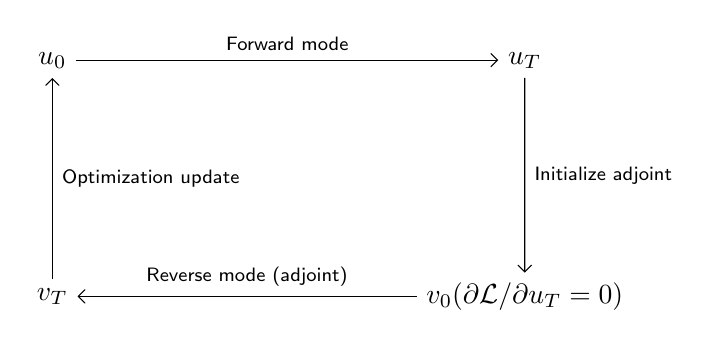
\begin{tikzpicture}[scale=3.0]
\node (A) at (0,1) {$u_0$};
\node (B) at (2,1) {$u_T$};
\node (C) at (2,0) {$v_0 (\partial \mathcal L/\partial u_T=0)$};
\node (D) at (0,0) {$v_T$};
\path[->,font=\scriptsize,>=angle 90]
(A) edge node[above]{Forward mode} (B)
(D) edge node[right]{Optimization update} (A)
(B) edge node[right]{Initialize adjoint} (C)
(C) edge node[above]{Reverse mode (adjoint)} (D);
\end{tikzpicture}
\end{center}
 \caption{Workflow for compression and restoring the solution.} 
  \label{fig:algorithm}
\end{figure}
\lstset{language=C,numbers=left,
    stepnumber=5,
    showstringspaces=false,
    tabsize=2,
    breaklines=true,
    breakatwhitespace=true}
\begin{lstlisting}[caption=PETSc code for PDE constrained optimization via adjoints, label=codemat]

  //TS object initialized previsouly
  ierr = TSSetSaveTrajectory(appctx->ts);CHKERRQ(ierr);
  ierr = TSSolve(appctx->ts,appctx->dat.curr_sol);CHKERRQ(ierr);
  
  // Compute the L2-norm of the objective function f
  ierr = VecDuplicate(appctx->dat.obj,&temp);CHKERRQ(ierr);
  ierr = VecCopy(appctx->dat.obj,temp);CHKERRQ(ierr);
  ierr = VecAXPY(temp,-1.0,appctx->dat.curr_sol);CHKERRQ(ierr);
  
  ierr   = VecDuplicate(temp,&temp2);CHKERRQ(ierr);
  ierr   = VecPointwiseMult(temp2,temp,temp);CHKERRQ(ierr);
  ierr = VecDot(temp2,appctx->SEMop.mass,f);CHKERRQ(ierr);

  // Initial conditions for the adjoint integration, given by 2*obj'=temp    
  ierr = VecScale(temp, -2.0);
  ierr = VecCopy(temp,appctx->dat.grad);CHKERRQ(ierr);
  
  //Set gradient and objective function
  ierr = TSSetCostGradients(appctx->ts,1,&appctx>dat.grad,NULL);CHKERRQ(ierr);
  
  ierr = TSAdjointSetUp(appctx->ts);CHKERRQ(ierr);
     
  //Solve adjoint step
  ierr = TSAdjointSolve(appctx->ts);CHKERRQ(ierr);
   
  ierr = VecCopy(appctx->dat.grad,G);CHKERRQ(ierr);
  
  //get solution status from TAO
  ierr=  TaoGetSolutionStatus(tao, &its, &ff, &gnorm, &cnorm, &xdiff, &reason);
\end{lstlisting}



\section{Validation and sources of error}

In the current section we illustrate...

\begin{figure}[!ht]
\centering
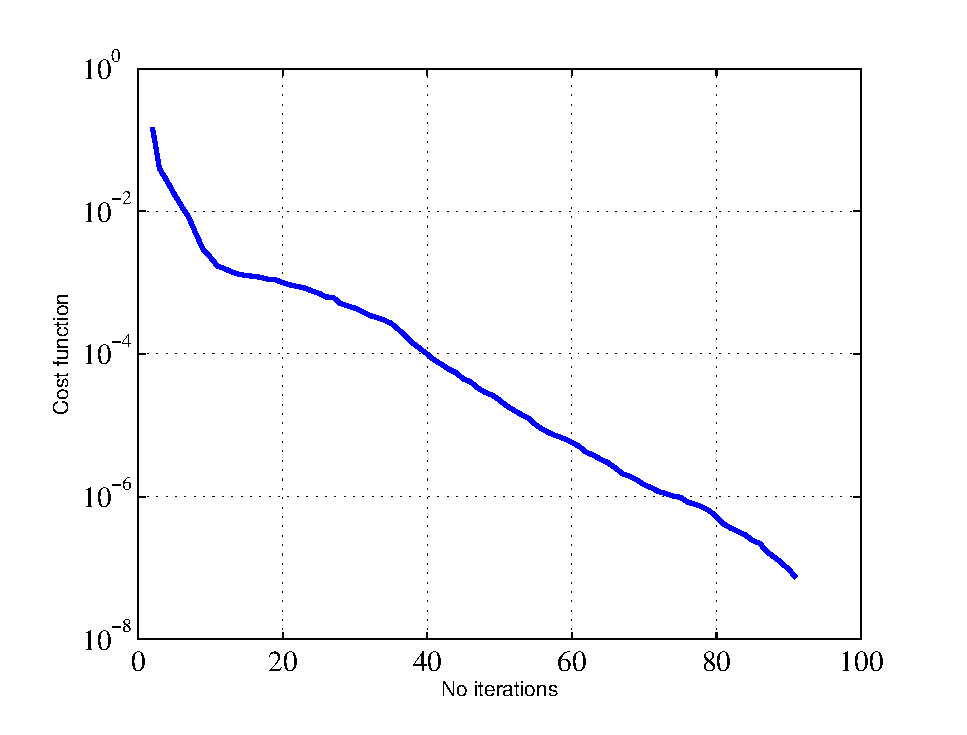
\includegraphics[width=0.47\textwidth]{Cost_decay.eps}
%\label{fig:wingfull_est}}
\caption{Cost function}
\end{figure}

\begin{figure}[!ht]
\centering
\subfloat[Initial condition(black) and desired profile(red)]
{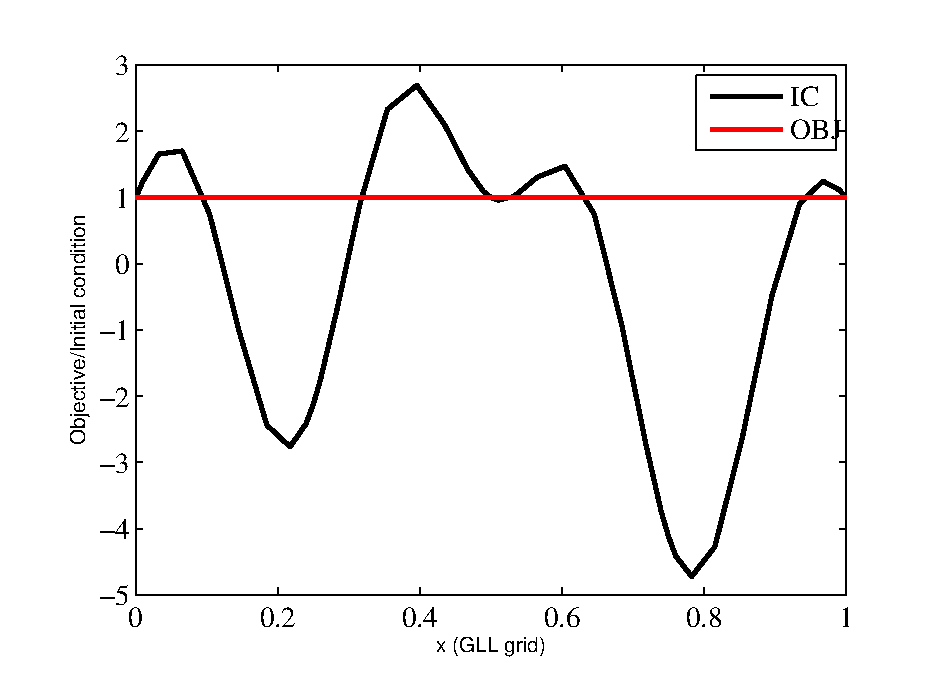
\includegraphics[width=0.47\textwidth]{IC_OBJ.eps}
\label{fig:wingfull_err}}
\quad
\subfloat[Gradient computed via finite differences(red), and gradient via adjoint computation(black), error between the two in max norm $0.435$.]
{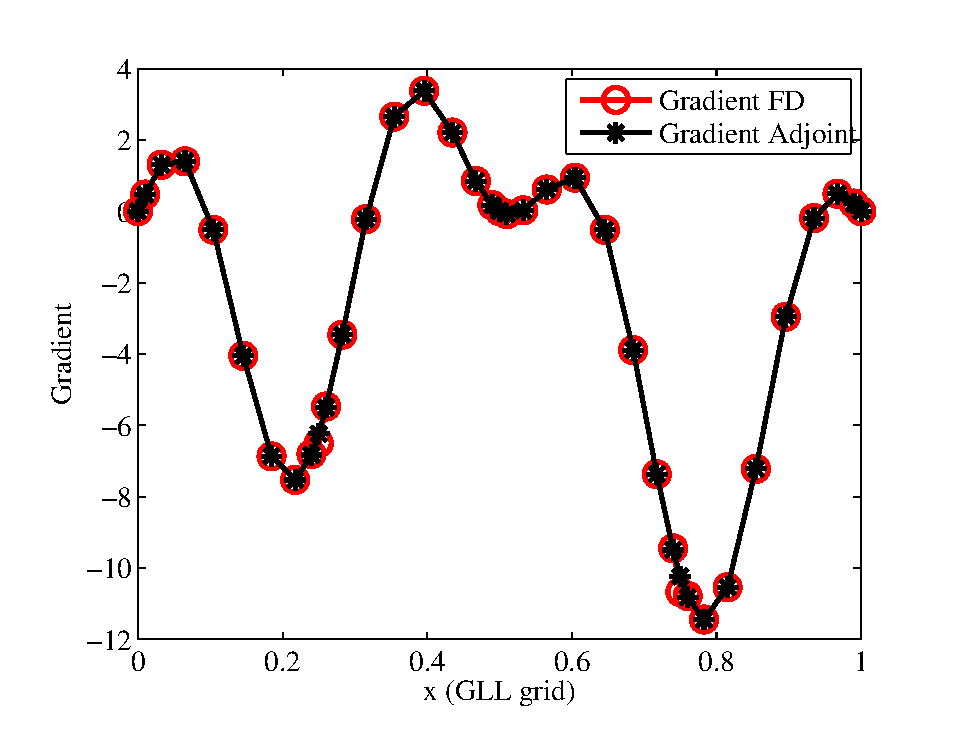
\includegraphics[width=0.47\textwidth]{Gradient.eps}
\label{fig:wingfull_est}}
\caption{Optimal initial conditions and gradient information}
\end{figure}



Sources of error
\begin{itemize}
\item Accumulation of local truncation error in the time-stepper
\item Inaccurate gradient information may hinder convergence


\end{itemize}



%
%\begin{figure}
%\begin{center}
% \begin{tikzpicture}[scale=2.0]
%\node (A) at (0,1) {$\mathbf u$};
%\node (B) at (1.5,1) {$T\mathbf u$};
%\node (C) at (1.5,0) {$T\tilde{\mathbf u}$};
%\node (D) at (0,0) {$\tilde{\mathbf u}$};
%\path[->,font=\scriptsize,>=angle 90]
%(A) edge node[above]{$DCT$} (B)
%(D) edge node[right]{$Error$} (A)
%(B) edge node[right]{$Truncate \rightarrow \texttt{Huffman\ encode}$} (C)
%(C) edge node[above]{$IDCT$} (D);
%\end{tikzpicture}
%\end{center}
% \caption{Workflow for compression and restoring the solution.} 
%  \label{fig:algorithm}
%\end{figure}
%
%\subsection{Algorithm}
%\begin{algorithm}
%\begin{algorithmic}[5]
%\Procedure{Setup}{}
%\State  {\tt T $\leftarrow$ DCT\_setup\_1d(p) }
%%\State {\tt M $\leftarrow$ build\_map($\text{mesh}_{\text{gll}})$}
%\EndProcedure
%\Procedure{Truncate}{}
%%\For {\tt k$\in$ $LocalEL_{id}(COMPnode)$} %\Comment{$ttotal$}
%\For { {\tt 0 $\leq$ k $<$ nel} }%\Comment{$ttotal$}
%%\State $u=M\cdot u$
%\State  {\tt $\text{u}_{\text{DCT,k}}=\text{T}\cdot \text{u}_\text{k} \cdot
%\text{T}^T \cdot \text{T}^T$} 
%\State { sort($\text{u}_{\text{DCT,k}}$)}
%%\State $\mathrm{u_{trunc}}=\mathrm{u_{DCT}}>\epsilon$
%\State {\tt$\text{u}_{\text{trunc,k}}=\text{u}_{\text{DCT,k}}>\epsilon$}
%\EndFor
%\EndProcedure
%\Procedure{Compress}{}
%\If {\tt IOnode} 
%\For {\tt q $\in$ IOchildren}
%\State {\tt Recv($\text{u}_{\text{trunc}}$,q)}
%\State {\tt $\text{u}_{\text{compress}}=$huff\_encode($\text{u}_{\text{trunc}}$)}
%\State {\tt output($\text{u}_{\text{compress}}$)}
%\EndFor
%\Else
%\State {\tt Send($\text{u}_{\text{trunc}}$,IOparent)}
%\EndIf
%\EndProcedure
%\end{algorithmic}
%\caption{Parallel compression on an already partitioned mesh with {\tt nel} elements
%each.}
%\label{alg:code_struct}
%\end{algorithm}
%
%\begin{figure}[!ht]
%\centering
%\subfloat[Compression ratio ($C_r$) vs error: (blue) GLL grid, (black) Chebyshev grid, 
%(green marker) corresponds to visualization in \reffig{fig:wingvis97}.]
%{\includegraphics[width=0.47\textwidth]{data/compvserrwing.eps}
%\label{fig:wingfull_err}}
%\quad
%\subfloat[A priori vs a posteriori error: (blue) GLL grid, (black) Chebyshev
%grid.]
%{\includegraphics[width=0.47\textwidth]{data/overestwing.eps}
%\label{fig:wingfull_est}}
%\caption{Flow past an airplane wing}
%\end{figure}

\section{Conclusions}
\label{sec:conclusion}


\section*{Acknowledgments}

This research used resources of the Argonne Leadership Computing Facility, 
which is a DOE Office of Science User Facility supported under Contract 
DE-AC02-06CH11357.


\vskip 10pt
%\begin{flushright}
\noindent\scriptsize \framebox{
%\parbox{3.2in}{
\parbox{0.96\textwidth}{
The submitted manuscript has been created by the University of Chicago
as Operator of Argonne National Laboratory (``Argonne'') under
Contract No. DE-AC02-06CH11357 with the U.S. Department of Energy.
The U.S. Government retains for itself, and others acting on its
behalf, a paid-up, nonexclusive, irrevocable worldwide license in said
article to reproduce, prepare derivative works, distribute copies to
the public, and perform publicly and display publicly, by or on behalf
of the Government.
}
} \normalsize
\newpage

\bibliographystyle{plain}
\bibliography{SEM_Petsc}
\end{document}

\begin{comment}

Set up the Lagrangian
$$\mathcal{L}[\vect u, \vect u_0]=\int_{\Omega}(\mathbf u[T]-\mathbf u_d[T])^2 \ \d \Omega +\int_0^T\int_{\Omega} P[\mathbf u] \mathbf v \ \d \Omega \d t + \int_0^T\int_{\Gamma} \mathbf v_b \mathbf (\mathbf u- \mathbf u_b) \ \d \Gamma \d t$$

Note: Chain rule for $f=g\circ h$, g must be Frechet and if h' is Frechet or gateaux so is f.

Note2: Riesz theorem: Let T be a functional on H then the Frechet derivative $T'(x)$ is given by
$T'(x) v= (\nabla T, v)$ for $\forall v \in H$.

Rewrite of the term
\begin{eqnarray}
\int_0^T\int_{\Omega} P[\mathbf u] \mathbf v \ \d \Omega \d t &=&
\int_0^T\int_{\Omega} \frac{\partial\mathbf u}{\partial t} \mathbf v \ \d \Omega \d t+ \int_0^T\int_{\Omega} \nu\Delta \mathbf u \cdot \mathbf v \ \d \Omega \d t+\int_0^T\int_{\Omega} \mathbf f(\mathbf x)  \mathbf v \ \d \Omega \d t \\ \nonumber
&=& \int_{\Omega}\mathbf u\mathbf v \ \d \Omega|_0^T -
\int_0^T\int_{\Omega}
 \frac{\partial\mathbf v}{\partial t} \mathbf u \ \d \Omega \d t+ \int_0^T\int_{\Gamma}(\nabla \mathbf u\cdot \mathbf v- \mathbf u\cdot \nabla\mathbf v)\mathbf n\ \d \Gamma \d t +
 \int_0^T\int_{\Omega} \nu\Delta \mathbf v\cdot  \mathbf u \ \d \Omega \d t+
 \int_0^T\int_{\Omega} \mathbf f(\mathbf x)  \mathbf v \ \d \Omega \d t \\ \nonumber
 &=& 
\int_0^T\int_{\Omega}
(- \frac{\partial\mathbf v}{\partial t}  +\nu\Delta \mathbf v)\cdot  \mathbf u\ \d \Omega \d t+\int_{\Omega}\mathbf u\mathbf v |_0^T \ \d \Omega
+ \int_0^T\int_{\Gamma}(\nabla \mathbf u\cdot \mathbf v- \mathbf u\cdot \nabla\mathbf v)\mathbf n\ \d \Gamma \d t +
 \int_0^T\int_{\Omega} \mathbf f(\mathbf x)  \mathbf v \ \d \Omega \d t \\ \nonumber
\end{eqnarray}

Grouping now the time dependent terms we have
\begin{eqnarray}
\mathcal{L}[\vect u, \vect u_0, \mathbf v]&=&\int_{\Omega}(\mathbf u[T]-\mathbf u_d[T])^2 +\mathbf u[T]\mathbf v[T]\ \d \Omega -\int_{\Omega}\mathbf u[0]\mathbf v[0]\ \d \Omega+\int_0^T\int_{\Omega} \overline{P}[\mathbf v] \mathbf u \ \d \Omega \d t + \\ \nonumber
 && \int_0^T\int_{\Gamma} \mathbf v_b \mathbf (\mathbf u- \mathbf u_b) \ \d \Gamma \d t +\int_0^T\int_{\Gamma}(\nabla \mathbf u\cdot \mathbf v- \mathbf u\cdot \nabla\mathbf v)\mathbf n\ \d \Gamma \d t +
 \int_0^T\int_{\Omega} \mathbf f(\mathbf x)  \mathbf v \ \d \Omega \d t 
\end{eqnarray}

\begin{eqnarray}
\frac{\partial L}{\partial \mathbf u}&=&- \frac{\partial\mathbf v}{\partial t}  +\nu\Delta \mathbf v \\
\frac{\partial L}{\partial \mathbf u_0}&=&-\mathbf v[0]\\
\frac{\partial L}{\partial \mathbf u_T}&=&2(\mathbf u[T]-\mathbf u_d[T])+\mathbf v[T]\\
\frac{\partial L}{\partial \mathbf u_b}&=&\\
\end{eqnarray}


\end{comment}

%%  LocalWords:  PDE PETSc Oana Constantinescu discretizations
%%  LocalWords:  Adjoint adjoint
